\chapter{Motivation for Classification Plan}
\section {Semisimple and unipotent elements}
{\bf Canonical group:}  $GL_n(q), q=p^k$ is a good prototype example of an ``almost simple" group.  Doing computations in
$GL_n(q)$ is also easier than doing them in $PSL_n(q)$.  There are two kinds of elements in $GL_n(q)$:
\emph{semisimple} elements are diagonalizable and have order co-prime to $p$ while 
\emph{unipotent} elements are upper (or lower) triangular and have centralizers
that are nilpotent. 
\\
\\
For example,
$$
s =\left(
\begin{array}{cc}
aI_r &  0_{r} \\
0_{n-r} &  bI_{n-r} \\
\end{array}
\right)
$$ is semisimple and its centralizer has the form
$$
C(s)=
\left(
\begin{array}{cc}
GL_r(q) &  0_{r} \\
0_{n-r} &  GL_{n-r}(q)\\
\end{array}
\right)
$$.  The element
$$
u =\left(
\begin{array}{ccc}
I_r &  0_{r} & 0_{r}\\
0_{n-2r} &  I_{n-2r} & 0_{n-2r}\\
I_r &  0_{r} & I_r\\
\end{array}
\right)
$$ is unipotent and its centralizer has the form
$$
C(u)=
\left(
\begin{array}{ccc}
X &  0_{r} & 0_r\\
P &  Y & 0_{n-2r}\\
Q & R & X\\
\end{array}
\right)
$$ which is nilpotent.  Further, 
$$
O_p(C(u))=
\left(
\begin{array}{ccc}
I_r &  0_{r} & 0_r\\
P &  I_{n-2r} & 0_{n-2r}\\
Q & R & I_r\\
\end{array}
\right)
$$.
\\
\\
Thus centralizers of semisimple elements are almost simple and have quasisimple components which
dominate the structure of $G$.  The centralizers of unipotent elements are dominated by a large 
normal $p$-group.  This motivates the definition of $E(G)$ we saw earlier.\\
\\
{\bf Definition:} $C_G(x)$ is in \emph{standard form} if $C_G(x)$ has one component, $L$, and $C_G(L)$ is small (often cyclic).
An example is $C_G(s)= GL_1(q) \times GL_{n-1}(q)$.  Finite simple groups can be determined by a centralizer in standard
form.
\begin{figure}
\center
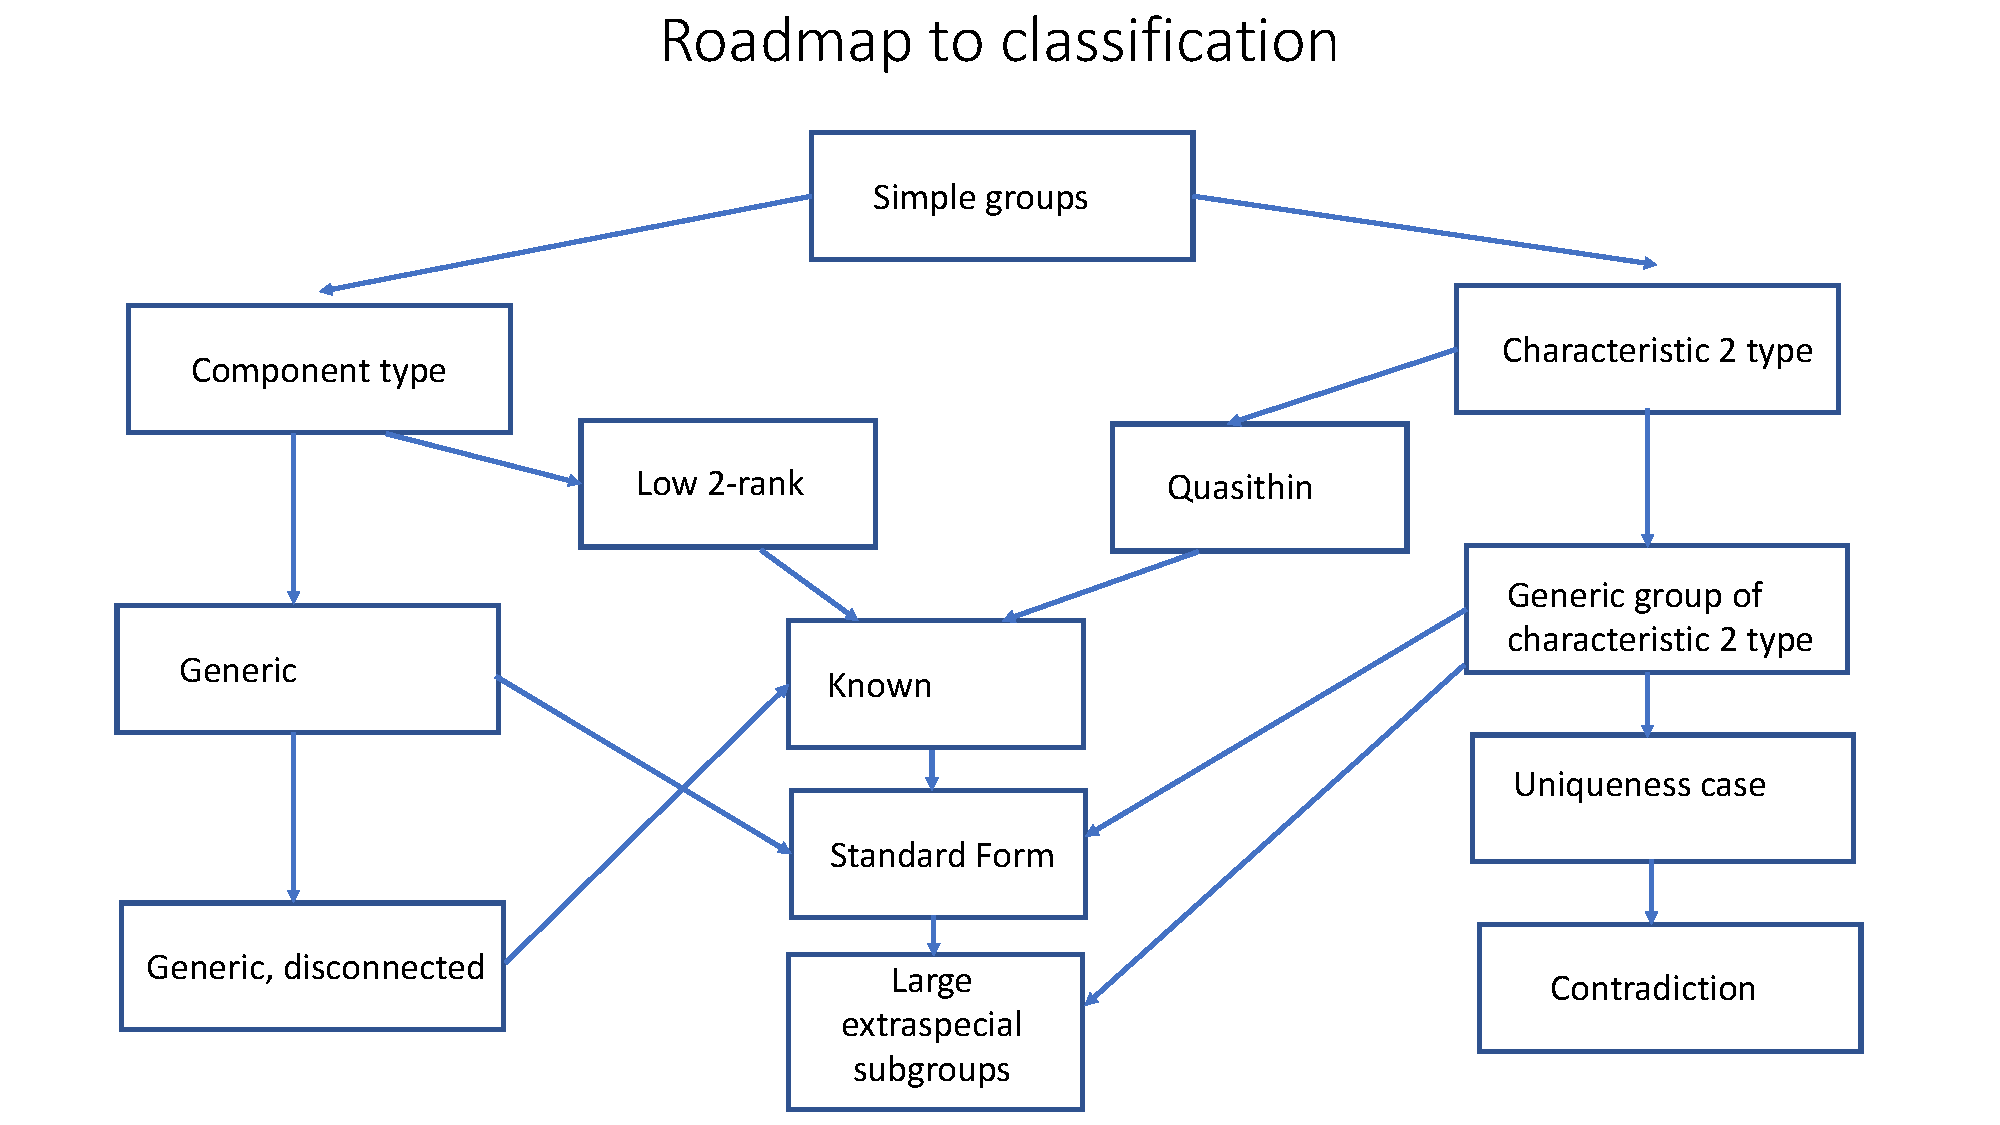
\includegraphics[width=0.7\textwidth,natwidth=642,natheight=610, height=70mm, width=80mm]{classificationroadmap.pdf}
\end{figure}
\\
\\
{\bf Theorem 1:} Let $G$ be a finite group with $O_{2'}(G)=1$, $s \in Inv(G)$ such that $G$ has one component, $L$
and $C_G(L)$ has a cyclic Sylow $2$-group then either (1) $G=C_G(x)$, (2) $H \leq G \leq Aut(H)$, $H$ simple, or (3)
$L \times L \leq G \leq Aut(L \times L)$, $L$, simple.
\\
\\
{\bf Theorem 2:} If $u$ is unipotent $C(u) \cap C(O_p(C(u))) \leq O_p(C(u))$.
\\
\\
{\bf Definition:} $G$ is of characteristic $p$-type if for all $p$ local subgroups, $H$, $C_H(O_p(H)) \leq O_p(H)$.
It is usually difficult to determine $G$ from $C(u)$ in characteristic $2$-type groups.  Lie groups of even characteristic
are of characteristic $2$-type.
\\
\\
{\bf Plan:} First we try to show the centralizer of an involution in $G$ is in standard form (i.e- is a Lie group of odd
characteristic or $A_{2k+1}$).  If not, $G$ is of characteristic $2$-type.  If $G$ is not of characteristic $2$-type, $G$
has an involution, $x$ and $C(x)/O(C(x))$ has a component.  This is a group of \emph{component} type.
\\
\\
{\bf Applying signalizers:}  What are the components of $C(a)/O(C(a))$, $a \in A^{\#}$.  Either $\theta(a)=O(C(a))$ is
an $A$-signalizer or for some $a,b \in A^{\#}$, there is a $b$-invariant component, ${\overline L}$ of
${\overline {C(a)}}= C(a)/O(C(a))$: $O(Aut_{\overline {C(a)}}({\overline L})) \cap C({\overline b}) \ne 1$.
\\
\\
{\bf Definition:} $G$ is \emph{balenced} if $O(C(x)) \leq O(G), x \in Inv(G)$.\\
\\
{\bf Unbalenced group conjecture:} Let $L \leq G \leq Aut(L)$, $L$, simple.   If $G$ is unbalenced
(1) $L$ is of Lie type with odd characteristic, (2) $L=A_{2k+1}$ or, $G=L_3(4), He$.
\\
\\
{\bf Component group conjecture:} Let $H$ be simple with $H \leq G \leq Aut(H)$, $x \in Inv(G)$.  Let ${\overline L}$
be a component of ${\overline {C(x)}} = C(x)/O(C(x))$ is known, then $G$ is a known simple group.\\
\\
Now let $G$ be a minimal counterexample then either $G$ is balenced or there is an unbalenced component, ${\overline L}$
is a quasi-simple group of unbalenced type.
\\
\\
{\bf Definition:} A quasisimple gropup, $L$, is a \emph{standard subgroup} of $G$, if $K=C_G(L)$ is tightly embedded in $G$,
$N_G(K)=N_G(L)$ and $L$ commutes with none of its conjugates.  $K$ is tightly embedded in $G$ if $|K|$ is even and $|K \cap K^g|$
is odd if $K^g \ne K$.
\\
\\
{\bf Standard Form Problem for $X$:}  If $H$ is simple, $H \leq G \leq Aut(H)$ and $L$ is a standard subgroup of $G$
with $L/Z(L) = H$ then $H$ is a known simple group.
\\
\\
{\bf Fisher:} $G$ is a finite group, ${\cal D}$ a collection of subgroups or elements permuted by conjugation, 
$G = \langle {\cal D} \rangle$.  Let $a,b \in {\cal D}$, $A$ and elementary abelian group of $q=p^e$,
$X= \langle a, b \rangle$, then $X$ is either (1) elementary abelian of order $q^2$, (2) isomorphic to $SL_2(q)$
or (3) if order $q^3$, $[a, b] \in {\cal D}$.  Originally, $q=1$ and (3) does not occur (like symplectic or unitary
groups over $GF(2)$ $|ab|=3$.  $M(22), M(23), M(24)'$ were found this way.
\\
\\
${\cal G}$ is a graph with vertex set ${\cal D}$.  $G(a)$ denotes the points adjacent to $a$.  $A^{\perp} = A \cup G(A)$.
${\cal G}^c$ is the complementary graph.
\\
\\
The \emph{triangle property} $A, B, C \in {\cal D}$, $C \in {\cal G}(A)$, $A, C \in {\cal G}^c(B)$. If $C$ is conjugate
to $A$ in $\langle \langle A, B, C \rangle \cap B^{\perp}$; this is like a $3$-transposition.
\\
\\
Let ${\cal G}$ and ${\cal G}^c$ be connected, $G$, simple, ${\cal D}$ is locally congugate ($[A, B] =1$ or $A \cong B$ in
$\langle A, B \rangle$) then $\langle A^{\perp}$ is transitive on ${\cal G}(A)$ and ${\cal G}^c(A)$ then $G$ has a rank $3$
permutation group.
\\
\\
Let ${\cal D}$ be a conjugacy class of $3$-transpositions and $G'$, simple.  Then ${\cal G}$ and ${\cal G}^c$ are connected
and $G$ is simple.
\\
\\
We want to show $x \in G, |x|=p$ with $C_G(X) = H$ in standard form with $O_{p'}(H)$ small.
\\
\\
{\bf $B_p$ Conjecture:} Let $G$ be a group with $O_{p'}(G)=1$ then for all $p$ elements, $x \in G$
$E(C(x)/(O_{p'}(C(x))) = E(C(x)) O_{p'}(C(x))/O_{p'}(C(x))$.
\\
\\
We use a signalizer to analyze $O_{p'}(H)$.  $\theta(A) \lhd G$.  Consider ${\cal D}(G, \Omega)$ with $A, B$ adjacent
iff $[A, B] = 1$.  For $B, D \in \Omega$ adjacent, $\theta(B)=\theta(BD)=\theta(D)$ then $\theta(A) = \theta(A)^g$ so
$\theta(A) \lhd G$.

